\section{Coulomb-Nuclear Interference}
\label{sec:coulomb}

The Coulomb-nuclear interference (CNI) can be used to\Break probe the nuclear component of the scattering amplitude. Since the CNI effects are sensitive to the phase of the nuclear amplitude, both modulus and phase can be tested. 

For the modulus, a relevant question is whether the earlier reported non-exponentiality of the differential\Break cross-section \cite{8tev-90m} can be attributed solely to the nuclear\Break component or whether Coulomb scattering gives a sizeable contribution. Concerning the phase, several parametrisations\Break with different physics interpretations will be tested; for each of them the $\rho$ parameter (representative for the phase value at $t = 0$ according to Eq.~(\ref{eq:rho def})) will be determined.

Section~\ref{sec:cni framework} outlines the theoretical concepts needed to describe the CNI effects. Section~\ref{sec:cni anal proc} provides details on fitting procedures used to analyse the data. Sections \ref{sec:fit exp1} and \ref{sec:fit exp3} discuss the fit results for two relevant alternatives in the description of the nuclear modulus: either exponential functions with exponents linear in $t$ (called ``purely exponential'') or exponential functions with higher-degree polynomials of $t$ in the exponent (called ``non-exponential'').


%----------------------------------------------------------------------------------------------------

\subsection{Theoretical Framework}
\label{sec:cni framework}

The amplitude describing elastic scattering of protons may be expected to receive three contributions, each corresponding to one of the following sets of Feynman diagrams.
\begin{itemize}
\item Containing QED elements only. This amplitude can be obtained by perturbative calculations, see Section~\ref{sec:cni coulomb}.
\item Containing QCD elements only. This amplitude is not directly calculable from the QCD lagrangian,\Break Sections~\ref{sec:cni nuclear modulus} and \ref{sec:cni nuclear phase} will propose several phenomenologically motived parame\-trisations.
\item Containing both QED and QCD elements. This contribution can neither be directly calculated from the Lagrangians, nor can \textit{ad hoc} parametrisations be used -- this amplitude is correlated with the previous two. Section~\ref{sec:cni interference} will introduce several interference formulae attempting to calculate the corresponding effects.
\end{itemize}

%------------------------------------------------------------------
\subsubsection{Coulomb Amplitude}
\label{sec:cni coulomb}
%
The Coulomb amplitude can be calculated from QED\Break (e.g.~\cite{block96}), using empirical electric ${\cal F}_{\rm E}$ and magnetic ${\cal F}_{\rm M}$ form factors of the proton. It can be shown (e.g.~Section 1.3.1 in~\cite{jan_thesis}) that, at low $|t|$, the effect of both form factors can be described by a single function ${\cal F}$:
\begin{equation}
\label{eq:coul cs}
	{\d\sigma^{\rm C}\over \d t} = {4\pi\alpha^2\over t^2}\,{\cal F}^4\ ,\ 
	{\cal F}^2 = {{\cal F}_{\rm E}^2 + \tau {\cal F}_{\rm M}^2\over 1 + \tau}\ ,\ 
	\tau = {|t|\over 4m^2}\ ,
\end{equation}
where $\alpha$ is the fine-structure constant and $m$ represents the proton mass.



%------------------------------------------------------------------
\subsubsection{Nuclear Amplitude -- Modulus}
\label{sec:cni nuclear modulus}

At $|t| \gtrsim 0.02\un{GeV^2}$ the effects due to the Coulomb interaction are not expected to be large (c.f.~Figure~\ref{fig:cni effect} or \cite{kklp11}). Thus, the measured cross-section can be attributed -- to a large extent -- to the nuclear component. Following Table~\ref{tab:data} and our previous publication \cite{8tev-90m} with high-precision data for $|t| < 0.2\un{GeV^2}$, the nuclear modulus will be parametrised as
\begin{equation}
\label{eq:nuc mod}
\left | {\cal A}^{\rm N}(t) \right | = \sqrt{s\over\pi} {p\over \hbar c} \sqrt{a} \exp\left( {1\over 2} \sum\limits_{n = 1}^{N_b} b_n\, t^n \right)\ ,
\end{equation}
where $N_b$ is the number of free parameters in the exponent. Consistently with \cite{8tev-90m} \footnote{%
Please note that Eq.~(15) in \cite{8tev-90m} contains a misprint: the exponent should have read $\sum\limits_{i=1}^{N_b} b_i\, |t|^i$.
}, the parameter $b_1$ gives the forward diffractive slope and $a$ the intercept of the differential cross-section at $t=0$. This parametrisation is also compatible with a number of theoretical models (see e.g.~\cite{elegent}).

Since the calculation of CNI may, in principle, involve integrations (e.g.~Eq.~(\ref{eq:int kl})), it is necessary to extend the nuclear amplitude meaningfully to $|t| > 0.2\un{GeV^2}$. Therefore the parametrisation Eq.~(\ref{eq:nuc mod}) is only used for $|t| < 0.2\un{GeV^2}$ while at $|t| > 0.5\un{GeV^2}$ the amplitude is fixed to follow a preliminary cross-section derived from the same data set as in \cite{8tev-90m} which features a dip-bump structure similar to the one observed at $\sqrt{s} = 7\un{TeV}$ \cite{epl95}. In order to avoid numerical problems, the intermediate region $0.2 < |t| < 0.5\un{GeV^2}$ is modelled with a continuous and smooth interpolation between the low and high-$|t|$ parts. It will be shown that altering the extended part of the nuclear amplitude\Break ($|t| > 0.2\un{GeV^2}$) within reasonable limits has negligible impact on the results presented later on.



%------------------------------------------------------------------
\subsubsection{Nuclear Amplitude -- Phase}
\label{sec:cni nuclear phase}

The following phase parametrisations are considered.

\begin{enumerate}

% ***
\item[a)]
A {\bf constant phase} is obviously the simplest choice:
\begin{equation}
\label{eq:nuc phase con}
\arg {\cal A}^{\rm N}(t) = {\pi\over 2} - \arctan\rho = \hbox{const} \quad .
\end{equation}
It leads to a strict proportionality between the real and the imaginary part of the amplitude at all $t$.
%This parametrisation is not compatible with Martin's theorem \cite{martin97} stating that, under some assumptions, the real part of an even-signature scattering amplitude must change sign at low $|t|$.

% ***
\item[b)]
The {\bf standard phase} parametrisation,
\begin{equation}
\label{eqn:nuc phase std}
	\begin{aligned}
		\arg {\cal A}^{\rm N}(t) =	& {\pi\over 2} - \arctan\rho + \arctan \left(\frac{|t|-|t_{0}|}{\tau}\right)\cr
									&- \arctan \left(\frac{-|t_{0}|}{\tau}\right) \: ,
	\end{aligned}
\end{equation}
describes the main features of many theoretical models -- almost imaginary amplitude in the forward direction ($\rho$ small) while almost purely real at the diffraction dip. The parameter values $t_0 = - 0.50\un{GeV^2}$ and $\tau = 0.1\un{GeV^2}$ have been chosen such that the shape is similar to a number of model predictions, see Figure~\ref{fig:phase illustration}.

% ***
\item[c)]
The parametrisation by {\bf Bailly et al.}~\cite{bailly87}:
\begin{equation}
\label{eq:nuc phase bai}
	\arg {\cal A}^{\rm N}(t) = {\pi\over 2} - \arctan {\rho\over 1 - {t\over t_{\rm d}}}
	%\arg {\cal A}^{\rm N}(t) = \arctan \left[ {1\over\rho} \left(1 - {t\over t_{\rm d}} \right) \right]\ ,
\end{equation}
where $t_{\rm d} \approx -0.53\un{GeV^2}$ gives the position of the diffractive minimum at $8\un{TeV}$ (preliminary result derived from the $\beta^* = 90\un{m}$ data \cite{8tev-90m}). This phase has a behaviour qualitatively similar to the model of Jenkovszky et al., see Figure~\ref{fig:phase illustration}.
%Like the constant phase, this parametrisation is not compatible with Martin's theorem~\cite{martin97}.

% ***
\item[d)]
Another parametrisation was proposed in \cite{kl94}:
\begin{equation}
\label{eq:nuc phase per}
\arg {\cal A}^{\rm N}(t) = {\pi\over 2} - \arctan\rho - \zeta_1 \left(- {t\over 1\un{GeV^2}} \right)^\kappa \e^{\nu t}\ .
\end{equation}
As shown in Figure~\ref{fig:phase illustration}, it features a peak at $t = -\kappa / \nu$ and for asymptotically increasing $|t|$ it returns to its value at $t=0$. Due to a potentially rapid variation at low $|t|$, this phase may yield a qualitatively different impact-parameter-space behaviour from the above parametrisations. In order to ensure fit stability the following parameters
\begin{equation}
\label{eq:nuc phase per val}
	\zeta_1 = 800\ ,\quad
	\kappa = 2.311\ ,\quad
	\nu = 8.161\un{GeV^{-2}}\ .
\end{equation}
have been fixed to values maintaining the desired impact-parameter behaviour at $\sqrt s = 8\un{TeV}$, using a method detailed in \cite{pk16}. This parametrisation with one free parameter will be denoted as {\bf peripheral phase} in what follows.

\end{enumerate}

\begin{figure*}
\begin{center}
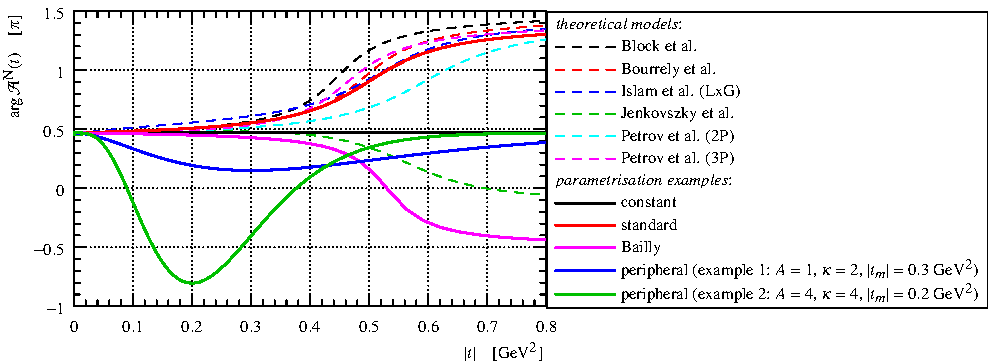
\includegraphics{fig/hadronic_phase_illustration.pdf}
\caption{Illustration of nuclear-phase forms. The dashed lines correspond to predictions by theoretical models (\cite{elegent} and references therein). The solid lines are typical examples of phases used in this report, all with the same value of $\rho = 0.10$. The peripheral example corresponds to the parameter values in Eq.~(\ref{eq:nuc phase per val}).
}
\label{fig:phase illustration}
\end{center}
\end{figure*}


Figure~\ref{fig:phase illustration} shows on the same plot a comparison of phase predictions by several models to typical examples of\Break parametrisations proposed above.

It should be noted that the nuclear phase has a strong influence on the amplitude behaviour in the space of impact parameter $b$ (for a detailed discussion see e.g.~Section~3 in~\cite{klk02}). A particularly decisive feature is the rate of phase variation at low $|t|$. Looking at Figure~\ref{fig:phase illustration} one can see that the constant, standard and Bailly phases are essentially flat at low $|t|$, thus leading to qualitatively similar pictures in the impact parameter space: elastic collisions being more central (preferring lower values of $b$) than the inelastic ones. Conversely, the peripheral phase parametrisation can yield a description with the opposite hierarchy, which is argued to be more natural by some authors (e.g. Section~4 in~\cite{kl96}). An impact-parameter study of the presented data will be given at end of Section~\ref{sec:fit exp3}.

%------------------------------------------------------------------
\subsubsection{Coulomb-Nuclear Interference Formulae}
\label{sec:cni interference}

The {\bf simplified West-Yennie formula (SWY)} \cite{wy68} was derived in the framework of perturbative quantum field theory by evaluating the lowest-order Feynman diagrams that comprise both nuclear and Coulomb interactions. In this approach, the interference is reduced to an additional phase between the Coulomb and nuclear amplitudes. Moreover, several approximations were used in the derivation. First, in order to avoid integrating over off-mass-shell contributions to the nuclear amplitude (essentially unknown), a very slow variation of the nuclear amplitude phase was assumed: $\arg {\cal A}^{\rm N} \approx \hbox{const}$. Then, in order to obtain a closed-form expression, the exponential slope of the nuclear modulus was assumed constant (i.e.~only the $b_1$ parameter is non-zero in the parametrisation Eq.~(\ref{eq:nuc mod})) which is formally incompatible with the existence of the diffractive minimum. The original formula did not contain the electromagnetic form factor ${\cal F}$, which was added later by hand:
\begin{equation}
\label{eq:int swy}
	\begin{aligned}
		{\d\sigma\over \d t}^{\rm C+N} =& {\pi (\hbar c)^2 \over s p^2} \left | {\alpha s\over t} {\cal F}^2 \e^{\I\alpha \Phi(t)} + {\cal A}^{\rm N}
			\right |^2\ ,\cr
		\Phi(t) =& - \left( \log {b_1 |t|\over 2} + \gamma \right)\ ,\cr
	\end{aligned}
\end{equation}
where $\alpha$ is the fine-structure constant and $\gamma \doteq 0.577$ the Euler constant. Despite the many limitations, the formula has been extensively used in past data analyses. For backward-comparison reasons it is also considered in this report.

The approach of {\bf Cahn} \cite{cahn82} uses an impact parameter formalism and is based on the additivity of eikonals. The first part of his derivation does not impose any limit on the nuclear amplitude, leading to the formula (Eq.~(30) in \cite{cahn82}):
\begin{equation}
\label{eq:int cahn}
	\begin{aligned}
		{\d\sigma\over \d t}^{\rm C+N} =& {\pi (\hbar c)^2 \over s p^2} \left | -{\alpha s\over q^2} {\cal F}^2
			+ {\cal A}^{\rm N}\, \Big[1 - \I\alpha G(-q^2)\Big] \right |^2\ ,\cr
		G(-q^2) =& - \int\limits_0^\infty \d q'^2 \log {q'^2\over q^2} {\d\phantom{q'^2}\over \d q'^2} {\cal F}^2(-q^2)\cr
				&+ {1\over\pi} \int\d^2 q' {{\cal F}^2(-q'^2)\over q'^2} \left[ {{\cal A}^{\rm N}\left(-[\vec{q} - \vec{q'}]^2\right) \over
					{\cal A}^{\rm N}(-q^2)} - 1 \right]\ , \cr
	\end{aligned}
\end{equation}
where $t=-q^2$, $\vec{q'}$ is a two-dimensional vector and $q'^2 = |\vec{q'}|^2$. The second part of the article gives simplified formulae for nuclear amplitudes with purely-exponential modulus and constant phase and is, thus, of limited interest for the present analysis.

{\bf Kundr\' at and Lokaj\' i\v cek (KL)} \cite{kl94} transformed the formula of Cahn, Eq.~(\ref{eq:int cahn}), into a form better suited for practical applications and added the kinematic limits on the momentum transfer:\footnote{%
Note that some recent publications by the same authors (e.g.~\cite{kl05,kklp11}) contain a misprint: the wrong sign in front of the second term contributing to $G(t)$.
}
\begin{equation}
\label{eq:int kl}
	\begin{aligned}
		{\d\sigma\over \d t}^{\rm C+N} =& {\pi (\hbar c)^2 \over s p^2} \left | {\alpha s\over t} {\cal F}^2
			+ {\cal A}^{\rm N}\, \Big[1 - \I\alpha G(t)\Big] \right |^2\ ,\cr
		G(t) =& \int\limits_{-4p^2}^0 \d t'\, \log {t'\over t} {\d\phantom{t'}\over \d t'} {\cal F}^2(t')\cr
			  &- \int\limits_{-4p^2}^0 \d t' \left( {{\cal A}^{\rm N}(t') \over {\cal A}^{\rm N}(t)} - 1 \right) { I(t, t')\over 2\pi }\ , \cr
		I(t, t') =& \int_0^{2\pi} \d\phi\ {{\cal F}^2(t'')\over t''}\ ,\cr
		t'' =& t + t' + 2\sqrt{t\, t'} \cos\phi\ .\cr
	\end{aligned}
\end{equation}
A slightly different variant proposed in Eq.~(22) in~\cite{kl05} was considered, too:
\begin{equation}
\label{eq:int kl exp}
	{\d\sigma\over \d t}^{\rm C+N} = {\pi (\hbar c)^2 \over s p^2} \left | {\alpha s\over t} {\cal F}^2
		+ {\cal A}^{\rm N}\, \e^{- \I\alpha G(t)} \right |^2 \ .
\end{equation}

The interference formula by Cahn, Eq.~(\ref{eq:int cahn}), and the KL formula, Eq.~(\ref{eq:int kl}), are very similar by construction and therefore they give practically identical interference effects.

Since the quantities $G$ in Eqs.~(\ref{eq:int cahn}) and (\ref{eq:int kl}) are complex, the interference effects in these treatments are generally more feature-rich than with the SWY formula, Eq.~(\ref{eq:int swy}), where the interference is reduced to a single additional phase $\Phi$.

By analysing Eqs.~(\ref{eq:int swy}), (\ref{eq:int cahn}) and (\ref{eq:int kl}), one can conclude that in the region where the nuclear amplitude dominates ($|t| \gtrsim 0.003\un{GeV^2}$), the effects due to the Coulomb interaction are of the order of $\alpha$ or the ratio $|{\cal A}^{\rm C}| / |{\cal A}^{\rm N}|$. In both cases, the magnitude of the interference effects can be expected at a percent level, as shown in Figure~\ref{fig:cni effect}. The figure also shows that the effects at different $|t|$ probe different parts of the nuclear phase: maximum sensitivity to $\rho$ lies at very low $|t|$ while at higher $|t|$ the effects are sensitive to phase values at slightly higher $|t|$. It can also be observed that for the constant, standard and Bailly phase the effects are very similar and rather mild at higher $|t|$. This can be understood from a very limited variation of the phase at low $|t|$, which is the region contributing most to the integral in Eq.~(\ref{eq:int cahn}) or (\ref{eq:int kl}). On the contrary, the higher $|t|$ response to peripheral phases can have various forms, often similar to the deviation of the reconstructed cross-section from pure-exponential, see the top plots in Figures~\ref{fig:fit exp1} and~\ref{fig:fit exp3}.

\begin{figure*}
\begin{center}
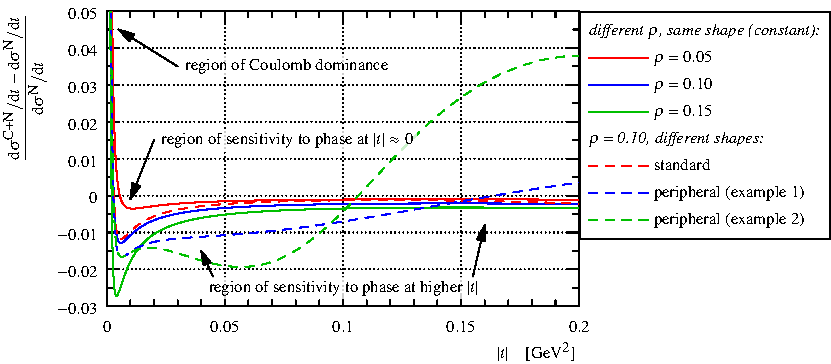
\includegraphics{fig/cni_effect_illustration.pdf}
\caption{%
Illustration of the effects due to the Coulomb interaction, using the KL formula. With the Cahn formula the plot looks identical. For the SWY formula, the picture is similar, however it misses the effects at $|t| \gtrsim 0.02\un{GeV^2}$. The curves show a response of the interference formula to different nuclear phases with a purely exponential nuclear modulus. The solid curves correspond to phases of the same shape (constant) but different values of $\rho$: the maximal response can be seen at $|t| \lesssim 0.01\un{GeV^2}$. Conversely, the dashed lines correspond to phases with fixed $\rho$ but various shapes (the same examples as in Figure~\ref{fig:phase illustration}): the response may be sizeable (e.g.~in the peripheral case) also at $|t| \gtrsim 0.02\un{GeV^2}$.
}
\label{fig:cni effect}
\end{center}
\end{figure*}


%----------------------------------------------------------------------------------------------------
\subsection{Analysis Procedure}
\label{sec:cni anal proc}

In addition to using the data from Table~\ref{tab:data}, one might consider including the $\beta^* = 90\un{m}$ data \cite{8tev-90m} which benefit from much smaller uncertainties. However, due to the limited\Break reach, $|t| \gtrsim 0.03\un{GeV^2}$, they have essentially no sensitivity to the $\rho$ parameter, cf.~Fig.~\ref{fig:cni effect}. Furthermore, due to possible systematic tensions between the data sets, the inclusion of the $\beta^* = 90\un{m}$ data may have a deteriorating impact on the $\rho$ determination. Therefore, the value of $\rho$ was determined from the $\beta^* = 1000\un{m}$ data only. For other parameters to which both data sets have non-negligible sensitivity (e.g.~$b_i$ in Eq.~(\ref{eq:nuc mod})), both data sets should give compatible results. This was verified for all the fits that will be presented later on. Since the $\beta^* = 90\un{m}$ data yield much lower uncertainties, both data sets have been used for determining all parameters except $\rho$. In practice, a series of two fits was performed:
\begin{enumerate}[leftmargin=2cm]
\item[step 1:] fit of $\beta^* = 1000\un{m}$ data with $\rho$ free,
\item[step 2:] fit of $\beta^* = 1000$ and $90\un{m}$ data with $\rho$ fixed from the preceding step.
\end{enumerate}

The standard least-squares method was used for all the fits. In particular, minimising
\begin{equation}
\label{eq:chi sq A}
	\begin{aligned}
		\chi^2 &= \Delta^\T \mat V^{-1} \Delta\ ,\quad
			\Delta_i = \left.{\d\sigma\over \d t}\right|_{{\rm bin}\ i} - {\d\sigma^{\rm C+N}\over\d t}\left(t^{\rm rep}_{{\rm bin}\ i}\right)\ ,\cr
		\mat V &= \mat V_{\rm stat} + \mat V_{\rm syst}\ ,\cr
	\end{aligned}
\end{equation}
where $\Delta$ is a vector of differences between the differential cross-section data and a fit function $\d\sigma^{C+N}/\d t$ evaluated at the representative point $t^{\rm rep}$ of each bin~\cite{lafferty94}. The minimisation is repeated several times, and the representative points are updated between iterations. The CNI effects are calculated using the computer code from~\cite{elegent}. The covariance matrix $\mat V$ has two components. The diagonal of $\mat V_{\rm stat}$ contains the statistical uncertainty squared from Table~\ref{tab:data} and from the Table~3 in \cite{8tev-90m}. $\mat V_{\rm syst}$ includes all systematic uncertainty contributions except the normalisation, see Eq.~(\ref{eq:covar mat}) and Eq.~(14) in \cite{8tev-90m}. For improved fit stability, the normalisation uncertainty is not included in the $\chi^2$ definition. Instead, the uncertainty is propagated for each fit parameter. For this purpose, the fit is repeated with $-1\un{\sigma}$, $0\un{\sigma}$ and $+1\un{\sigma}$ biases independently in: global normalisation ($1\un{\sigma} = 4.2\un{\%}$), $90\un{m}$ data normalisation ($0.08\un{\%}$) and $1000\un{m}$ data normalisation ($0.25\un{\%}$). This gives a sample of 27 fit results, from which one can estimate the propagated normalisation uncertainty of a parameter as $(\hbox{max} - \hbox{min})/2$, where ``max'' (``min'') is the greatest (smallest) value in the sample. This normalisation uncertainty is, at the end, added quadratically to the uncertainty reported by the fit with no bias.


The fits have shown low sensitivity to several of the\Break choices presented above, summarised in the following list. 
\begin{itemize}
\item Choice of the form factor in Eq.~(\ref{eq:coul cs}). The options considered in \cite{elegent} have been tested, none of them giving any significant difference with respect to the default choice \cite{puckett10}.
\item Extension of the modulus of the nuclear amplitude to the unobserved $|t|$ region, see the last paragraph in Section~\ref{sec:cni nuclear modulus}. No effect was observed when the high-$|t|$ part was altered (both shape and normalisation) nor when the size of the transition region was changed.
\item Use of the Cahn or KL formula. Only the latter will be used in what follows to represent both of them.
\item The two variants of the KL formula, Eqs.~(\ref{eq:int kl}) and (\ref{eq:int kl exp}). The latter will be used below.
\item Fits with constant, standard and Bailly phase are practically indistinguishable. This can be expected from\Break Fig.~\ref{fig:cni effect} showing that the corresponding CNI effects are very similar. Therefore, in the remainder of this article, these phases will be treated as a single family represented by the constant phase.
\end{itemize}


One of the goals of this study is to probe the origin of the differential cross-section non-exponentiality reported earlier~\cite{8tev-90m}. Therefore, the following two classes of fits were considered.
\begin{itemize}
\item Section \ref{sec:fit exp1}: fits with purely exponential nuclear modulus, that is $N_b=1$ in Eq.~(\ref{eq:nuc mod}). In this case, the non-exponentiality can come from the CNI effects only.
\item Section \ref{sec:fit exp3}: fits with nuclear modulus flexible enough to describe the non-exponentiality without the CNI effects. Here, the non-exponentiality may be due to the nuclear modulus, CNI effects or both.
\end{itemize}
For each of these nuclear modulus cases, the following two phase parametrisations were considered:
\begin{itemize}\setlength\itemsep{0pt}
\item constant phase, Eq.~(\ref{eq:nuc phase con}), as a representative of the\Break central-phases family,
\item peripheral phase, Eq.~(\ref{eq:nuc phase per}) with parameters fixed to the values in Eq.~(\ref{eq:nuc phase per val}) to represent peripheral behaviour in the impact parameter space.
\end{itemize}

In each case, the fit results are used to calculate the total cross-section via the optical theorem:
\begin{equation}
\label{eq:si tot}
\sigma_{\rm tot}^2 = {16\pi\, (\hbar c)^2\over 1 + \rho^2}\, a\ .
\end{equation}
Note that unlike all previous total cross-section determinations at LHC, in this article all the ingredients come consistently from a single analysis.


%----------------------------------------------------------------------------------------------------
\subsection{Fits with Purely Exponential Nuclear Modulus}
\label{sec:fit exp1}

The goal of this section is to test whether the data are compatible with a purely exponential nuclear modulus, i.e.~$N_b=1$ in Eq.~(\ref{eq:nuc mod}). In other words, the non-exponentiality is\Break forced to originate from the Coulomb-induced effects. The fit results obtained with the KL and (where applicable) SWY formulae are summarised in Table~\ref{tab:fit exp1} and graphically shown in Fig.~\ref{fig:fit exp1}.

\begin{table*}
\caption{Fit results with $N_b=1$. Each column corresponds to a fit with different interference formula and/or nuclear phase.}
%\vskip-3mm
\label{tab:fit exp1}
\begin{center}
\setlength\tabcolsep{2.5mm}
%\small
\input fig/fit_exp1/table_data.tex
\end{center}
\end{table*}

\begin{figure*}
\begin{center}
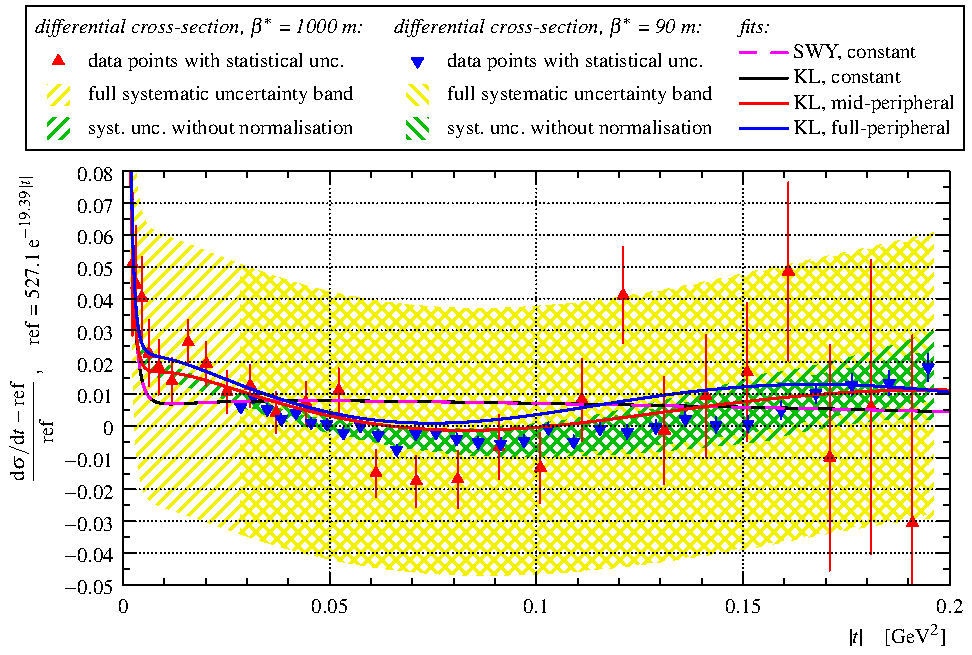
\includegraphics{fig/fit_exp1/t_dist_rel_with_fit.pdf}
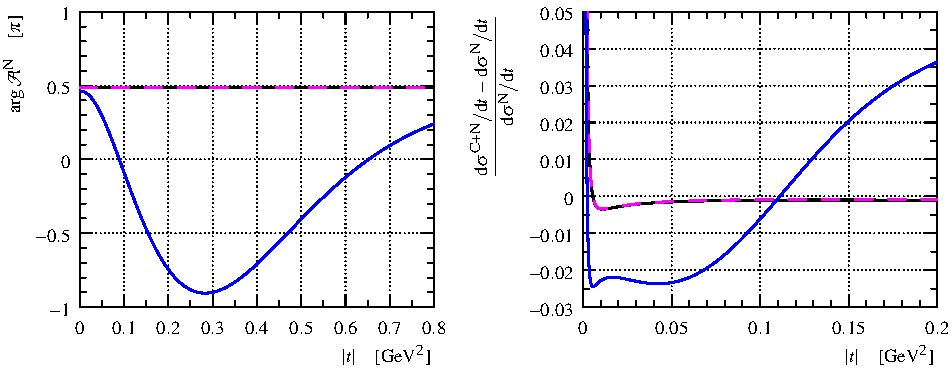
\includegraphics{fig/fit_exp1/phase_cni_effect.pdf}
\caption{Visualisation of the fit results from Table~\ref{tab:fit exp1} obtained with $N_b=1$. The continuous (dashed) lines correspond to fits with Cahn or KL (SWY) formula. Note that the fits with constant nuclear phase largely overlap.
TOP: fits compared to differential cross-section data in a relative reference frame, see the vertical axis label. The reference is identical to the one in \cite{8tev-90m}. 
BOTTOM LEFT: $t$-dependence of the nuclear phase as extracted from the fits.
BOTTOM RIGHT: the effects induced by the Coulomb interaction for each of the fits.
}%
\label{fig:fit exp1}
\end{center}
\end{figure*}

Table~\ref{tab:fit exp1} shows that both fits with constant phase are essentially identical and have bad quality. The step-2 fit using both $\beta^*=1000$\,m and $90\un{m}$ data can be excluded with $7.6\un{\sigma}$ significance. Consequently, since the combination of $N_b=1$ and constant phase is the only one compatible with the SWY approach, that formula is experimentally excluded even on the basis of only the low-$|t|$ data set discussed here. This result is complementary to the observation of a diffractive minimum at $\sqrt{s} = 8\un{TeV}$ (to be published in a forthcoming article) which also contradicts the assumptions of the SWY formula.

Although the quality of the fit with the peripheral phase is good, this option seems disfavoured from different perspectives.
\begin{itemize}
\item There are several theoretical reasons for the nuclear component not to be purely exponential, e.g.~\cite{kmr00-multiPom,kmr12-opacity,kmr15-slope,fagundes15}. Indeed, most elastic scattering models predict\Break a non-exponential nuclear modulus, see e.g.~\cite{elegent} and references therein.
\item The value of $\rho$ obtained in this fit may be regarded as an outlier with respect to a consistent pattern of other fits from this article and extrapolations from lower energies: e.g.~\cite{fagundes12,block12,compete} and most models in \cite{elegent}.
\end{itemize}
Let us also recall that the good quality of this fit is possible due to the more complex KL formula where the CNI effects go beyond a simple additional phase in the traditional SWY concept.


%----------------------------------------------------------------------------------------------------
\subsection{Fits with Non-Exponential Nuclear Modulus}
\label{sec:fit exp3}

The aim of this section is to discuss fits with enough flexibility in the nuclear modulus to describe the non-exponentiality in the data. Since a non-exponential hadronic modulus is used, the only applicable interference formula is KL. $N_b=2$ to $5$ were considered. The optimal degree was chosen according to two criteria: reasonable $\chi^2/\hbox{ndf}$ and stability of fit parameters (among which $\rho$ is one of the most sensitive). For instance, with constant phase the fit (step 1) with $N_b=2$ yields $\chi^2/\hbox{ndf} = 1.07$ and $\rho = 0.10$ while the one with $N_b=3$ gives $\chi^2/\hbox{ndf} = 1.03$ and $\rho = 0.12$. Both fits have the normalised $\chi^2$ reasonably close to $1$, but the value of $\rho$ changes significantly between $N_b=2$ and $3$ which is unexpected should $N_b=2$ be sufficient. On the other hand $N_b=4$ gives $\chi^2/\hbox{ndf} = 0.861$ which is unreasonably low. Therefore $N_b=3$ was chosen.

\iffalse
* KL, exp2, con
\rh       =   0.101 \pm  0.026
last fit     : chi^2/ndf = 68.45/57 = 1.201, probability = 1.42E-01, significance = 1.467, quality = 0.000000
previous fit : chi^2/ndf = 27.74/26 = 1.067, probability = 3.71E-01, significance = 0.894

* KL, exp3, con
\rh       =   0.121 \pm  0.029
last fit     : chi^2/ndf = 57.59/56 = 1.028, probability = 4.16E-01, significance = 0.813, quality = 0.000000
previous fit : chi^2/ndf = 25.63/25 = 1.025, probability = 4.27E-01, significance = 0.794

* KL, exp4, con
rho    =   0.087 +-  0.034
last fit     : chi^2/ndf = 54.48/55 = 0.990, probability = 4.95E-01, significance = 0.683, quality = 0.000000
previous fit : chi^2/ndf = 20.66/24 = 0.861, probability = 6.59E-01, significance = 0.442
\fi

As shown in Table~\ref{tab:fit exp3}, both fits have reasonable fit quality and remarkably consistent values of $\rho$ (identical within the resolution) which are compared to previous determinations at lower energies in Fig.~\ref{fig:rho cmp exp3}. Take note that the obtained parameters for the nuclear amplitude ($a$ and $b_i$) are consistent between step 1 ($\beta^* = 1000\un{m}$ data only) and step 2 (both $\beta^* = 1000$ and $90\un{m}$ data) of the fitting procedure as already mentioned in Section~\ref{sec:cni anal proc}.

Fig.~\ref{fig:fit exp3} shows that the level of Coulomb-induced effects is very different in the fits. It is much stronger in the case of the peripheral-phase, which can be expected as this phase features a faster variation in the low-$|t|$ region.


\begin{table*}
\caption{Fit results with Cahn or KL formula and $N_b=3$.}
%\vskip-3mm
\label{tab:fit exp3}
\begin{center}
\setlength\tabcolsep{5mm}
%\small
\input fig/fit_exp3/table_data.tex
\end{center}
\end{table*}

\begin{figure*}
\begin{center}
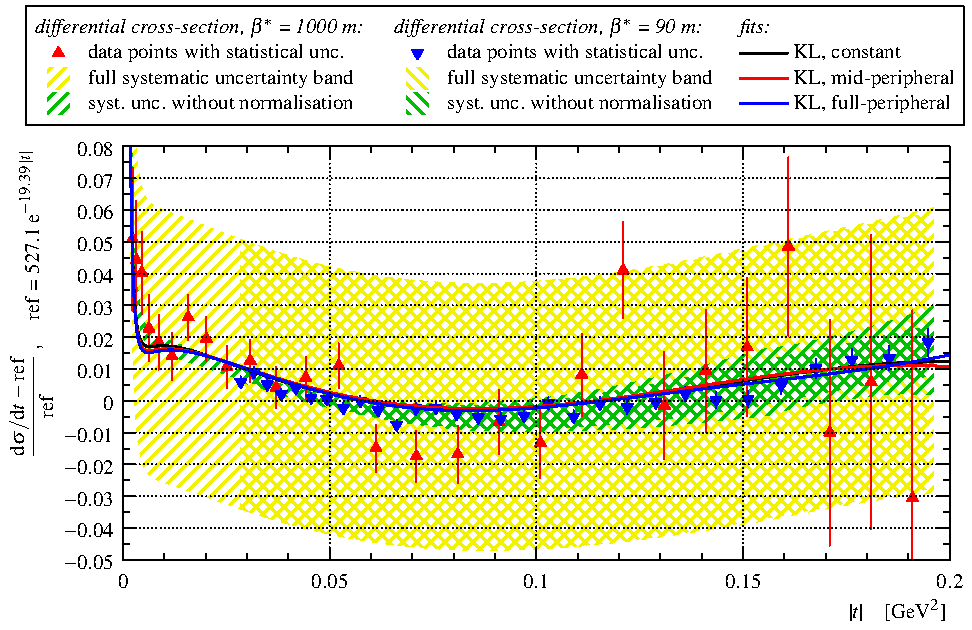
\includegraphics{fig/fit_exp3/t_dist_rel_with_fit.pdf}
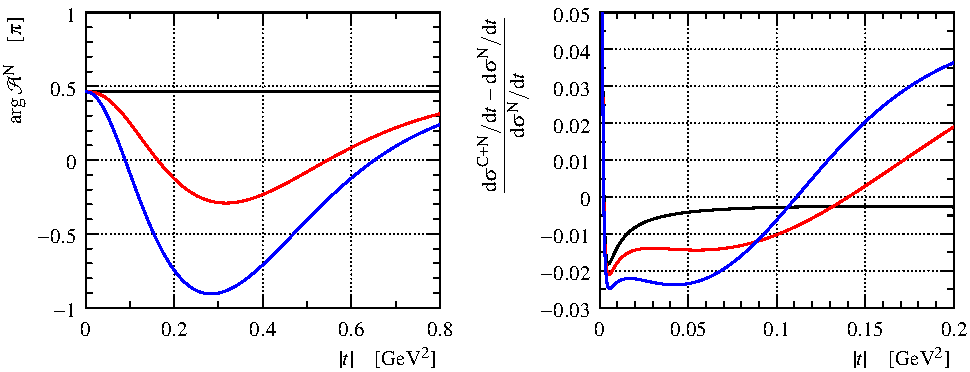
\includegraphics{fig/fit_exp3/phase_cni_effect.pdf}
\caption{Visualisation of the fit results from Table~\ref{tab:fit exp3} obtained with Cahn or KL formula and $N_b=3$. The solid lines correspond to fits with different nuclear phases.
TOP: fits compared to differential cross-section data in a relative reference frame, see the vertical axis label. The reference is identical to the one in \cite{8tev-90m}. 
BOTTOM LEFT: $t$-dependence of the nuclear phase as extracted from the fits.
BOTTOM RIGHT: the effects induced by the Coulomb interaction for each of the fits.
}%
\label{fig:fit exp3}
\end{center}
\end{figure*}


\begin{figure}
\begin{center}
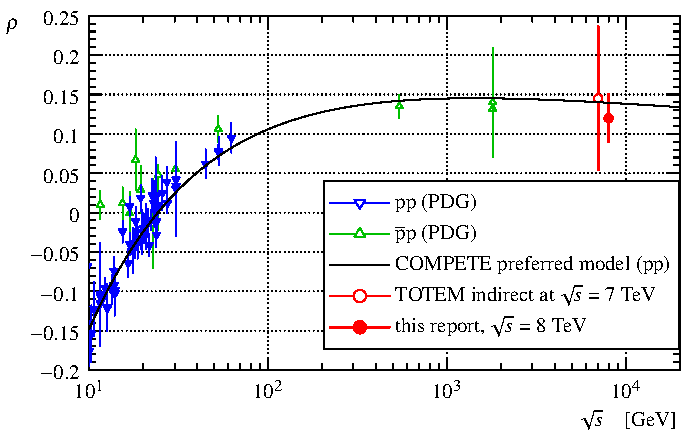
\includegraphics{fig/rho_s.pdf}
\caption{Energy dependence of the $\rho$ parameter. The blue (green) triangles correspond to $\rm pp$ ($\rm \bar pp$) data from PDG \cite{pdg} -- note that most of these points were determined with the help of the SWY formula, shown to be inconsistent with the present data. The hollow red circle stands for the earlier indirect determination by TOTEM~\cite{epl101-tot}. The filled red circle represents the two results from Table~\ref{tab:fit exp3} which are numerically identical within the resolution. The black curve gives the preferred $\rm pp$ model by COMPETE~\cite{compete}, obtained without using LHC data.
}%
\label{fig:rho cmp exp3}
\end{center}
\end{figure}


The total cross-section results from the two fits in Table~\ref{tab:fit exp3} are well consistent with each other and also with previous measurements \cite{8tev-90m,prl111}. The slightly higher values with respect to previous analyses neglecting the Coulomb interaction are expected as long as $\rho > 0$. This gives negative interference at low $|t|$ and when separated leads to an increase of nuclear cross-section intercept $a$ and thus also total cross-section via Eq.~(\ref{eq:si tot}).


It is interesting to study the fit behaviour in the impact-parameter space. The scattering amplitude in this representation (sometimes called profile function), ${\cal P}(b)$, can be obtained from the nuclear amplitude by means of\Break Fourier-Bessel transformation (see e.g.~\cite{klk02}):
\begin{equation}
\label{eq:prof fun}
	\begin{aligned}
		&{\cal P}(b) = {1\over 4 p \sqrt s} \int\limits_{-\infty}^0 \d t\,J_0\left(b\sqrt{-t}\over \hbar c\right)\,{\cal A}^{\rm N}(t)\ ,\cr
		&\hbox{normalised that } {\sigma_{\rm el} = 8\pi \int\limits_0^{+\infty} b\, \d b\, |{\cal P}(b)|^2}\ ,\cr
	\end{aligned}
\end{equation}
where $\sigma_{\rm el}$ is the integrated elastic cross-section. The profile functions for the two fits from Table~\ref{tab:fit exp3} are shown in Figure~\ref{fig:bdist exp3}. The fit with constant nuclear phase gives a distribution peaked at $b=0$. It corresponds to a behaviour that is more central than for the fit with peripheral phase, where the amplitude modulus reaches maximum at $b\approx 1.2\un{fm}$. These considerations can be extended to inelastic channels. Following Section~3 in~\cite{klk02}, one can calculate the mean values of $b^2$ for elastic ($\langle b^2\rangle_{\rm el}$), inelastic ($\langle b^2\rangle_{\rm inel}$) or all ($\langle b^2\rangle_{\rm tot}$) collisions:
\begin{equation}
\label{eq:ms b}
	\begin{aligned}
		\langle b^2\rangle_j &= {
			\int b\,\d b\,b^2\, h_j(b)
			\over
			\int b\,\d b\, h_j(b)
		}\ ,\qquad h_{\rm el}(b) = |{\cal P}(b)|^2\cr
		h_{\rm tot}(b) &= \Im {\cal P}(b)\ ,\qquad
		h_{\rm inel}(b) = h_{\rm tot}(b) - h_{\rm el}(b)\ .\cr
	\end{aligned}
\end{equation}
Their values reproduced in Figure~\ref{fig:bdist exp3} indicate that the fit with constant nuclear phase leads to a picture with elastic collisions more central than the inelastic ones. The hierarchy is inverted for the fit with peripheral phase.

\begin{figure}
\begin{center}
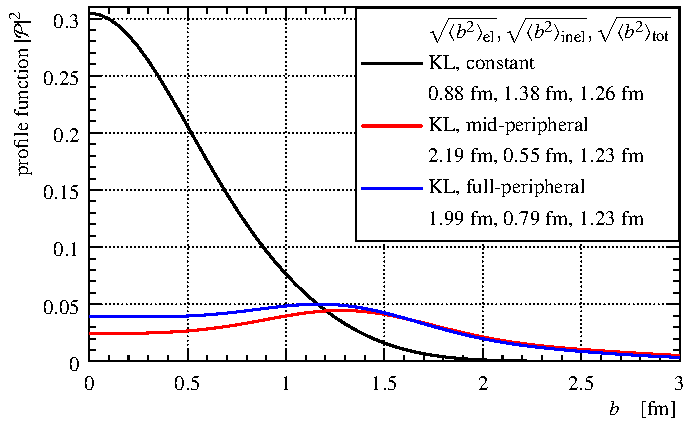
\includegraphics{fig/fit_exp3/b_dist.pdf}
\caption{%
Square of the impact-parameter amplitude, ${\cal P}$, as a function of impact parameter, $b$. The two lines correspond to the fits in Table~\ref{tab:fit exp3}, using the same colour code as in Figure~\ref{fig:fit exp3}. The root-mean-squares of $b$ in the legend are calculated from Eq.~(\ref{eq:ms b}).
}%
\label{fig:bdist exp3}
\end{center}
\end{figure}
